% PTE Core 模考 3B —— 口语 错题与详解·整理卷  版本 000（自包含）
% 编译: xelatex 本文件.tex   （需 Noto CJK + TeX Gyre Heros 字体）
% 本版本含图片，依赖同目录的 img/ 子目录。
\documentclass[11pt]{article}

% --------- 样式（原 ptestyle.sty，已内联）---------
% ============================================================
%  ptestyle.sty  —  PTE 模考错题整理卷 共享样式
%  编译引擎: XeLaTeX  (中英混排, 需要 Noto CJK 字体)
% ============================================================

\usepackage[a4paper,margin=2cm,headsep=4mm]{geometry}
\usepackage{fontspec}
\usepackage{xeCJK}
\usepackage[table]{xcolor}
\usepackage[normalem]{ulem}        % \sout 删除线
\usepackage{tabularx}
\usepackage{array}
\usepackage{ragged2e}
\usepackage{enumitem}
\usepackage[most]{tcolorbox}
\usepackage{fancyhdr}
\usepackage{graphicx}
\usepackage{pifont}                % \ding{51}=✓ \ding{55}=✗（阅读对错标注）
\usepackage{needspace}
\usepackage{tikz}

% ---------- 字体 ----------
\setmainfont{TeX Gyre Heros}            % 拉丁: Helvetica 风格(纤细清晰)
\setCJKmainfont{Noto Sans CJK SC}
\setCJKsansfont{Noto Sans CJK SC}
\newfontfamily\cjkserif{Noto Serif CJK SC}
\linespread{1.18}
\setlength{\parindent}{0pt}
\setlength{\parskip}{4pt}

% ---------- 配色 ----------
\definecolor{cWrong}{HTML}{D32F2F}     % 红  = 修改 / 错误
\definecolor{cFix}{HTML}{1B7F3B}       % 绿  = 正确建议
\definecolor{cDelete}{HTML}{1565C0}    % 蓝  = 删除
\definecolor{cInsert}{HTML}{7B1FA2}    % 紫  = 插入
\definecolor{cPartial}{HTML}{E07B00}   % 橙  = 部分得分
\definecolor{cNote}{HTML}{0277BD}      % 蓝  = 注解
\definecolor{cAccent}{HTML}{16A085}    % 主题青绿(平台主色)
\definecolor{cWrongBg}{HTML}{FBE0E0}
\definecolor{cDelBg}{HTML}{DCE8FB}
\definecolor{cInsBg}{HTML}{EEE0F5}
\definecolor{cHead}{HTML}{20303A}
\definecolor{cGrayBox}{HTML}{F4F6F7}
\definecolor{cModelBg}{HTML}{EAF7EF}
\definecolor{cYouBg}{HTML}{FFF7F5}
\definecolor{cNoteBg}{HTML}{EAF3FA}
\definecolor{cRule}{HTML}{D7DEE2}

% ---------- 行内批改宏 (复刻平台标注) ----------
% \fix{原词}{正确}  红色删除线 + 绿色上标改正  (修改/拼写/空格)
\newcommand{\fix}[2]{%
  \colorbox{cWrongBg}{\textcolor{cWrong}{\sout{#1}}}%
  \,\textsuperscript{\textcolor{cFix}{\footnotesize #2}}}
% \del{原词}  蓝色删除线  (应删除)
\newcommand{\del}[1]{%
  \colorbox{cDelBg}{\textcolor{cDelete}{\sout{#1}}}%
  \,\textsuperscript{\textcolor{cDelete}{\footnotesize 删}}}
% \ins{词}  紫色下划线  (应插入)
\newcommand{\ins}[1]{%
  \textsuperscript{\textcolor{cInsert}{\footnotesize $\wedge$}}%
  \colorbox{cInsBg}{\textcolor{cInsert}{#1}}}
% \miss{词}  灰色删除线  (口语漏读 / 未作答)
\newcommand{\miss}[1]{\textcolor{gray}{\sout{#1}}}
% \add{原词}{改正}  橙色波浪线 + "补"标签  (平台漏标、本卷补标的错误)
\definecolor{cAdd}{HTML}{E65100}
\newcommand{\add}[2]{%
  \textcolor{cAdd}{\uwave{#1}}%
  \,\textsuperscript{\textcolor{cAdd}{\footnotesize 补：#2}}}
% 高亮(口语发音): 好/中/差
\newcommand{\spk}[2]{\textcolor{#1}{#2}}

% ---------- 评分单元格着色 ----------
\newcommand{\sfull}[1]{\textcolor{cFix}{\bfseries #1}}     % 满分
\newcommand{\spart}[1]{\textcolor{cPartial}{\bfseries #1}} % 部分
\newcommand{\szero}[1]{\textcolor{cWrong}{\bfseries #1}}   % 零/低分

% ---------- 分数小标签 ----------
\newtcbox{\chip}[1][cAccent]{on line, boxsep=2pt, left=4pt, right=4pt, top=1pt,
  bottom=1pt, arc=3pt, colback=#1, colframe=#1, coltext=white, nobeforeafter,
  fontupper=\bfseries\footnotesize}

% ---------- 题块小标题 ----------
\newcommand{\ptesub}[1]{%
  \par\needspace{2\baselineskip}\smallskip
  {\color{cAccent}\rule[-0.2ex]{3pt}{1.05em}}\hspace{6pt}%
  {\bfseries\color{cHead}#1}\par\nopagebreak\smallskip}

% ---------- 题块外框 ----------
% \begin{qblock}{标号·题型}{右上信息(得分/用时)} ... \end{qblock}
\newtcolorbox{qblock}[2]{
  breakable, enhanced, arc=2.5pt,
  colback=white, colframe=cRule, boxrule=0.6pt,
  left=11pt, right=11pt, top=8pt, bottom=10pt,
  toptitle=3pt, bottomtitle=3pt, lefttitle=11pt, righttitle=11pt,
  colbacktitle=cHead, coltitle=white, fonttitle=\bfseries,
  title={#1\hfill\normalfont\bfseries\small #2}}

% ---------- 文本块: 题干 / 范文 / 你的作答 / 建议 ----------
\newtcolorbox{promptbox}{enhanced, breakable, colback=cGrayBox, colframe=cGrayBox,
  arc=2pt, left=8pt, right=8pt, top=6pt, bottom=6pt, boxrule=0pt}
\newtcolorbox{modelbox}{enhanced, breakable, colback=cModelBg, colframe=cModelBg,
  borderline west={3pt}{0pt}{cFix}, arc=1pt, left=8pt, right=8pt, top=6pt, bottom=6pt, boxrule=0pt}
\newtcolorbox{youbox}{enhanced, breakable, colback=cYouBg, colframe=cYouBg,
  borderline west={3pt}{0pt}{cWrong}, arc=1pt, left=8pt, right=8pt, top=6pt, bottom=6pt, boxrule=0pt}
\newtcolorbox{notebox}{enhanced, breakable, colback=cNoteBg, colframe=cNoteBg,
  borderline west={3pt}{0pt}{cNote}, arc=1pt, left=8pt, right=8pt, top=6pt, bottom=6pt, boxrule=0pt}

% ---------- 评分表 ----------
% 用法见正文; 这里给表头宏
\newcommand{\scorehead}{%
  \rowcolors{2}{cGrayBox}{white}
  \arrayrulecolor{cRule}}

% ---------- 章节大标题 ----------
\newcommand{\ptesection}[3]{% #1=中文名 #2=英文名 #3=该项分数
  \addcontentsline{toc}{section}{#1}%
  \needspace{6\baselineskip}
  \begin{tcolorbox}[enhanced, colback=cAccent, colframe=cAccent, sharp corners,
     left=14pt, right=14pt, top=10pt, bottom=10pt, boxrule=0pt]
    {\fontsize{20}{24}\selectfont\bfseries\color{white} #1\ \ }%
    {\large\color{white!85} #2}\hfill
    {\large\color{white}本项得分\ \ }{\fontsize{22}{24}\selectfont\bfseries\color{white} #3}%
    \ {\color{white!85}/ 90}
  \end{tcolorbox}}

% ---------- 题型小节分隔 (口语 RA/RS/DI/RTS/ASQ 等) ----------
\newcommand{\ptetask}[2]{%
  \addcontentsline{toc}{subsection}{#1\ #2}%
  \needspace{4\baselineskip}\medskip
  \begin{tcolorbox}[enhanced, colback=cHead, colframe=cHead, sharp corners,
     left=12pt, right=12pt, top=5pt, bottom=5pt, boxrule=0pt]
    {\large\bfseries\color{white} #1}\ \ {\color{white!80} #2}
  \end{tcolorbox}\smallskip}

% ---------- 口语 AI 语音识别着色 (复刻平台: 优/良/差 + 停顿) ----------
\definecolor{cSpkGood}{HTML}{2E9E5B}   % 优 绿
\definecolor{cSpkOk}{HTML}{C77F00}     % 良 黄/琥珀
\definecolor{cSpkBad}{HTML}{E0352B}    % 差 红
\newcommand{\sg}[1]{\textcolor{cSpkGood}{#1}}   % 优
\newcommand{\sy}[1]{\textcolor{cSpkOk}{#1}}     % 良
\newcommand{\sr}[1]{\textcolor{cSpkBad}{#1}}    % 差
\newcommand{\smiss}[1]{\textcolor{cSpkBad}{\sout{#1}}}  % 漏读 (红删除线)
\newcommand{\pse}{{\color{gray}\,/\,}}          % 停顿
\newcommand{\asrlegend}{{\footnotesize\color{gray}AI 语音识别\quad
  {\color{cSpkGood}\textbullet}\,优\ \ {\color{cSpkOk}\textbullet}\,良\ \
  {\color{cSpkBad}\textbullet}\,差\ \ {\color{gray}/}\,停顿\ \
  {\color{cSpkBad}\sout{词}}\,漏读}}
\newtcolorbox{asrbox}{enhanced, breakable, colback=white, colframe=cRule,
  boxrule=0.6pt, arc=1pt, left=8pt, right=8pt, top=6pt, bottom=6pt}

% ---------- 中文翻译行 ----------
\newcommand{\zh}[1]{{\footnotesize\textcolor{cNote}{\textbf{译}}\ \textcolor{gray}{#1}}}

% ---------- 阅读填空 / 选择 对错标注 ----------
\newcommand{\rok}[1]{{\color{cFix}\ding{51}\,#1}}                 % 选对(绿勾 + 词)
\newcommand{\rno}[2]{{\color{cWrong}\ding{55}\,\sout{#1}}\,{\footnotesize\color{cFix}(答案:\,#2)}}  % 选错: 你的(红删) + (答案:正确)
\newcommand{\rblank}[1]{{\color{cFix}\underline{\,#1\,}}}         % 直接给空的正确答案(无你的作答时)

% ---------- 听力专用 ----------
\newcommand{\hiw}[2]{{\color{cWrong}\uline{#1}}\,{\footnotesize\color{cFix}(听:#2)}} % HIW: 屏幕错词(红下划线)+ 实际读音
\newcommand{\lhit}[1]{{\color{cFix}#1}}                           % WFD: 命中的词(绿)
\newcommand{\lmiss}[1]{{\color{cWrong}\sout{#1}}}                 % WFD: 多余/错误的词(红删, 1B 配色)
% ---- WFD 逐词批改 · 本套 2B 平台配色（与 1B 相反）：绿=命中 / 红括号=漏写 / 灰删除线=多写或听错 ----
% 说明: 2B 平台把"漏写"标红(加括号)、"多写/听错"标灰删除线; 本卷忠于原图按此复刻。
\newcommand{\womit}[1]{{\color{cWrong}(#1)}}                      % WFD: 漏写(正确答案有、你没写)——红色括号
\newcommand{\wbad}[1]{{\color{gray}\sout{#1}}}                    % WFD: 多写/听错(你写了但错)——灰删除线
\newcommand{\wfdlegend}{{\footnotesize\color{gray}WFD 配色：\
  {\color{cFix}命中}\ \ {\color{cWrong}(漏写)}\ \ {\color{gray}\sout{多写/听错}}}}

% ---------- 颜色图例 ----------
\newcommand{\ptelegend}{%
  \begin{tcolorbox}[enhanced, colback=cGrayBox, colframe=cRule, boxrule=0.5pt,
    arc=2pt, left=10pt, right=10pt, top=6pt, bottom=6pt]
  {\bfseries\color{cHead}颜色说明\quad}
  \fix{改}{正}~修改/拼写\quad
  \del{删}~应删除\quad
  \ins{插}~应插入\quad
  \add{补}{改正}~平台漏标(本卷补标)\quad
  {\color{cFix}\rule{1em}{0.6em}}~范文/正确\quad
  {\color{cNote}\rule{1em}{0.6em}}~AI 建议
  \end{tcolorbox}}

% ---------- 页眉页脚 ----------
\pagestyle{fancy}
\fancyhf{}
\renewcommand{\headrulewidth}{0.4pt}
\renewcommand{\footrulewidth}{0pt}
\fancyhead[L]{\footnotesize\color{cHead}\bfseries PTE Core 模考 3B}
\fancyhead[R]{\footnotesize\color{gray} 错题与详解整理卷}
\fancyfoot[C]{\footnotesize\color{gray}\thepage}

\begin{document}

% --------- 封面（原 cover.tex）---------
% ---------- 封面 / 成绩总览 ----------
\definecolor{mListen}{HTML}{1F3A5F}
\definecolor{mRead}{HTML}{C2D70B}
\definecolor{mSpeak}{HTML}{4D4D4D}
\definecolor{mWrite}{HTML}{A01B7D}

\begin{titlepage}
\thispagestyle{empty}
\centering
\vspace*{1.4cm}

{\fontsize{30}{36}\selectfont\bfseries\color{cHead} PTE Core 模考 3B}\\[4mm]
{\fontsize{17}{20}\selectfont\color{cAccent}\bfseries 错题与详解 · 整理卷}\\[3mm]
{\color{gray} APEUni / 猩际 PTE 模考　·　提交时间 2026-07-05 13:36}\\[1.2cm]

% ---- 总分 ----
\begin{tcolorbox}[width=0.62\textwidth, halign=center, enhanced,
  colback=cAccent, colframe=cAccent, arc=6pt, boxrule=0pt, top=10pt, bottom=10pt]
  {\color{white}\large 总分 Overall}\\[2pt]
  {\fontsize{46}{50}\selectfont\bfseries\color{white} 53}
\end{tcolorbox}

\vspace{1.0cm}

% ---- 四项分数条形图 ----
\begin{tcolorbox}[width=0.84\textwidth, enhanced, colback=white, colframe=cRule,
  boxrule=0.8pt, arc=4pt, left=18pt, right=18pt, top=14pt, bottom=14pt]
\setlength{\tabcolsep}{6pt}\renewcommand{\arraystretch}{1.7}
\sffamily
\begin{tabular}{@{}r@{\hskip 8pt}l@{\hskip 10pt}l@{}}
 \bfseries Listening 听力 & {\color{mListen}\rule{6.11cm}{0.42cm}} & {\bfseries\large 55}\\
 \bfseries Reading 阅读   & {\color{mRead}\rule{4.67cm}{0.42cm}}   & {\bfseries\large 42}\\
 \bfseries Speaking 口语  & {\color{mSpeak}\rule{4.67cm}{0.42cm}}  & {\bfseries\large 42}\\
 \bfseries Writing 写作   & {\color{mWrite}\rule{8.11cm}{0.42cm}}  & {\bfseries\large 73}\\
\end{tabular}\\[2mm]
{\footnotesize\color{gray} 满分 90　|　刻度: 条长 = 得分 / 90}
\end{tcolorbox}

\vfill
\begin{flushleft}\small\color{gray}
\textbf{说明:}本卷由本次模考的题目与"详解"截图逐题誊写、重新排版而成,完整保留每道题的
\emph{题干 / 原文、范文、你的作答、逐项评分、彩色批改与 AI 中文建议}。\\
所有错误按平台标注用颜色标出(见下方图例)。原始"详解"PDF 不可复制、仅截图,本卷内容均为人工对照誊录,若与原图有出入以原图为准。
\end{flushleft}
\vspace{4mm}
\ptelegend
\end{titlepage}

% --------- 口语正文（原 sec_speaking_body.tex）---------
% ===================== 口语 Speaking =====================
\ptesection{口语}{Speaking · 5 题型}{42}

\vspace{1mm}
{\small\color{gray} 本部分共 \textbf{30 题}：\textbf{RA 朗读}Q1--7、\textbf{RS 复述句子}Q8--18、\textbf{DI 描述图}Q19--21、\textbf{RTS 情景应答}Q22--24、\textbf{ASQ 简短回答}Q25--30。每题保留\textbf{正确文本／范文}、\textbf{你的作答（AI 语音识别逐词配色）}与平台\textbf{逐项评分}，并附\textbf{中文翻译}。平台「AI 语音识别」按发音质量\textbf{逐词上色}，本卷逐词复刻。RA／RS 的上色对象是\textbf{原文／原句}；DI／RTS 的上色对象是\textbf{你说出的话（语音识别原文，含口误照原样保留）}；RS 额外用\textbf{红色删除线}标记漏读/未读出的词。
本套口语总分 \textbf{42 / 90}：RA 内容维度普遍满分，失分集中在发音与流利度；RS 失分主要在大段漏读；RTS/DI 的恰当性/内容尚可，发音流利度偏低；ASQ 6 题全部未答对。}

\vspace{1mm}
{\small\color{gray}\textbf{配色图例：}\asrlegend}
\vspace{2mm}

\ptetask{朗读}{Read Aloud · RA　Q1--7（内容除 Q1 为 4.44/5 外均 5/5，失分主要在发音／流利度）}
% ---------------- Q1 ----------------
\begin{qblock}{Q1\quad RA \#771\ \ Venture Capitals}{朗读 · 总分 \textcolor{cAccent}{\bfseries 20}/90}
\ptesub{原文 Text（朗读对象）}
\begin{promptbox}
Venture capitals and public funding authorities need to carefully consider the incentive issues of entrepreneurs when providing support. In allocating resources to potentially competing innovators, there is a trade-off between the risk of innovation failure and rent dissipation: diverse investment lowers the risk of having no successful innovation but also reduces the expected profit from the post-innovation market.
\end{promptbox}
\zh{风险投资机构和公共资助机构在提供支持时，需要认真考虑创业者的激励问题。在向可能相互竞争的创新者分配资源时，存在创新失败风险与租金耗散之间的权衡：分散投资降低了完全没有成功创新的风险，但也降低了创新后市场的预期利润。}
\ptesub{你的朗读（AI 语音识别逐词配色）}
\asrlegend
\begin{asrbox}
\sr{Venture} \sr{capitals} \sg{and} \sg{public} \sr{funding} \sg{authorities} \sg{need} \sy{to} \sr{carefully} \sg{consider} \sg{the} \sr{incentive} \sg{issues} \sg{of} \sr{entrepreneurs} \sg{when} \sg{providing} \sg{support} \sg{In} \sr{allocating} \sg{resources} \sy{to} \sr{potentially} \sg{competing} \sr{innovators} \pse \sg{there} \sg{is} \sg{a} \sg{trade} \sy{off} \sg{between} \sg{the} \sy{risk} \sg{of} \sg{innovation} \sr{failure} \sg{and} \sy{rent} \sg{dissipation} \pse \sy{diverse} \sg{diverse} \sg{the} \sg{the} \sr{investment} \sr{lowers} \sg{the} \sy{risk} \sg{of} \sr{having} \sg{no} \sr{successful} \pse \sr{innovation} \sg{but} \sg{also} \sr{reduces} \sg{the} \sr{expected} \sr{profit} \sr{from} \sy{the} \sg{post} \sr{innovation} \sr{market}
\end{asrbox}
\smallskip
{\small\textbf{评分：}内容 \sfull{4.44/5} \quad\textperiodcentered\quad 发音 \spart{25/90} \quad\textperiodcentered\quad 流利度 \szero{18/90}}\quad{\footnotesize\color{gray}（用时 01:10）}
\end{qblock}

% ---------------- Q2 ----------------
\begin{qblock}{Q2\quad RA \#763\ \ Peptic Ulcer}{朗读 · 总分 \textcolor{cAccent}{\bfseries 14}/90}
\ptesub{原文 Text（朗读对象）}
\begin{promptbox}
The most common peptic ulcer symptom is burning stomach pain. Stomach acid makes the pain worse, as does having an empty stomach. The pain can often be relieved by eating certain foods that buffer stomach acid or by taking an acid-reducing medication, but then it may come back. The pain may be worse between meals and at night.
\end{promptbox}
\zh{消化性溃疡最常见的症状是胃部灼痛。胃酸会使疼痛加剧，空腹时也是如此。进食某些能中和胃酸的食物，或服用抑酸药物，通常可以缓解疼痛，但疼痛可能会再次出现。疼痛在两餐之间及夜间可能会加重。}
\ptesub{你的朗读（AI 语音识别逐词配色）}
\asrlegend
\begin{asrbox}
\sg{The} \sg{most} \sg{common} \sr{peptic} \pse \sr{ulcer} \sr{symptom} \sy{is} \sr{burning} \sr{stomach} \sg{pain} \sr{Stomach} \sg{acid} \sr{makes} \sg{the} \sg{pain} \sy{worse} \pse \sg{as} \sg{does} \sg{having} \sy{an} \pse \sg{empty} \sr{stomach} \sg{the} \pse \sg{The} \pse \sg{pain} \sg{can} \sg{often} \sg{be} \sr{relieved} \pse \sg{be} \sg{eating} \sr{by} \sr{eating} \sr{certain} \sr{foods} \sy{that} \sy{buffer} \sr{stomach} \sr{acid} \sy{or} \sg{by} \sg{taking} \sy{an} \pse \sr{acid} \sr{reducing} \sr{medication} \pse \sg{but} \sg{then} \pse \sg{it} \sg{may} \sg{come} \sg{back} \sg{The} \sr{pain} \sg{may} \sg{be} \sy{worse} \sg{between} \sy{meals} \sg{and} \sg{at} \sg{night}
\end{asrbox}
\smallskip
{\small\textbf{评分：}内容 \sfull{5/5} \quad\textperiodcentered\quad 发音 \szero{17/90} \quad\textperiodcentered\quad 流利度 \szero{11/90}}\quad{\footnotesize\color{gray}（用时 01:07）}
\end{qblock}

% ---------------- Q3 ----------------
\begin{qblock}{Q3\quad RA \#762\ \ Topic}{朗读 · 总分 \textcolor{cAccent}{\bfseries 33}/90}
\ptesub{原文 Text（朗读对象）}
\begin{promptbox}
When you have selected a topic, you will first have to familiarize yourself with the topic in order to clarify it. In this way you will get a clearer idea of all aspects concerning the topic, definitions, facts and theories. You will get to know related terms and concepts, the context and the various possible ways of approaching the topic.
\end{promptbox}
\zh{选定题目之后，你首先需要熟悉这个题目，以便把它弄清楚。这样你就能更清楚地了解与该题目相关的各个方面——定义、事实和理论。你也会由此了解相关的术语和概念、背景，以及探讨这个题目的各种可能方式。}
\ptesub{你的朗读（AI 语音识别逐词配色）}
\asrlegend
\begin{asrbox}
\sg{When} \sg{you} \sg{have} \sg{selected} \sg{a} \sg{topic} \pse \sg{you} \sg{will} \sg{first} \sg{have} \sg{to} \sy{familiarize} \sy{yourself} \sg{with} \sg{the} \sy{topic} \sg{in} \sg{in} \sg{order} \sg{to} \sg{clarify} \sy{it} \sg{In} \sg{this} \sg{way} \sg{you} \sg{will} \sg{get} \sg{a} \sy{clearer} \sg{idea} \sy{of} \pse \sg{all} \sy{aspects} \pse \sy{concerning} \sy{the} \sg{topic} \pse \sy{definitions} \pse \sy{facts} \sg{and} \sy{theories} \sg{You} \sg{will} \sg{get} \sr{to} \sg{know} \sg{to} \sg{related} \sy{terms} \sg{and} \sg{concepts} \pse \sg{the} \sr{context} \sg{and} \sg{the} \sy{various} \sg{possible} \sy{ways} \sy{of} \sg{approaching} \sg{the} \pse \sg{topic}
\end{asrbox}
\smallskip
{\small\textbf{评分：}内容 \sfull{5/5} \quad\textperiodcentered\quad 发音 \spart{34/90} \quad\textperiodcentered\quad 流利度 \spart{32/90}}\quad{\footnotesize\color{gray}（用时 01:09）}
\end{qblock}

% ---------------- Q4 ----------------
\begin{qblock}{Q4\quad RA \#759\ \ Beauty}{朗读 · 总分 \textcolor{cAccent}{\bfseries 31}/90}
\ptesub{原文 Text（朗读对象）}
\begin{promptbox}
Beauty is subjective, and as such it of course cannot be defined in absolute terms. But we all know or feel when something is beautiful to us personally. And in such instances, methods of physics and network science can be used to quantify and help us better understand what it is that evokes that pleasant feeling.
\end{promptbox}
\zh{美是主观的，因此当然无法用绝对的标准来定义。但我们都能知道或感受到某样事物对自己而言是否美。在这种情况下，可以借助物理学和网络科学的方法来量化，并帮助我们更好地理解到底是什么唤起了那种愉悦的感觉。}
\ptesub{你的朗读（AI 语音识别逐词配色）}
\asrlegend
\begin{asrbox}
\sg{Beauty} \sg{is} \sy{subjective} \pse \sg{and} \sg{as} \sg{such} \sy{it} \sg{of} \sg{course} \sg{cannot} \sg{be} \sy{defined} \sg{in} \sy{absolute} \sg{terms} \sg{But} \sg{we} \sg{all} \sg{know} \sg{or} \sg{feel} \sg{when} \sg{something} \sg{is} \sy{beautiful} \sg{to} \sy{us} \sy{personally} \sg{And} \sg{in} \sg{such} \sy{instances} \pse \sr{methods} \sg{of} \sr{physics} \sg{and} \sy{network} \sg{science} \pse \sg{can} \sg{be} \sg{used} \sg{to} \sg{quantify} \sg{and} \sg{and} \sy{help} \sg{us} \sg{better} \sy{understand} \sg{what} \sg{it} \sg{is} \sg{that} \pse \sy{evokes} \sy{that} \sg{pleasant} \sy{feeling}
\end{asrbox}
\smallskip
{\small\textbf{评分：}内容 \sfull{5/5} \quad\textperiodcentered\quad 发音 \spart{36/90} \quad\textperiodcentered\quad 流利度 \spart{24/90}}\quad{\footnotesize\color{gray}（用时 01:13）}
\end{qblock}

% ---------------- Q5 ----------------
\begin{qblock}{Q5\quad RA \#758\ \ Biodiversity Decline}{朗读 · 总分 \textcolor{cAccent}{\bfseries 36}/90}
\ptesub{原文 Text（朗读对象）}
\begin{promptbox}
Climate change and biodiversity decline are major challenges of our time. Both are predominantly caused by human activities, with profound consequences for people and the ecosystems on which we depend. Some actions we can undertake are beneficial in both areas, helping to mitigate and adapt to climate change as well as conserve and restore biodiversity.
\end{promptbox}
\zh{气候变化和生物多样性衰退是我们这个时代的重大挑战。两者主要都是由人类活动造成的，给人类以及我们所依赖的生态系统带来深远影响。我们可以采取的一些行动在这两个方面都有益处，既有助于减缓和适应气候变化，也有助于保护和恢复生物多样性。}
\ptesub{你的朗读（AI 语音识别逐词配色）}
\asrlegend
\begin{asrbox}
\sy{Climate} \sg{change} \sg{and} \sg{biodiversity} \sg{decline} \sg{are} \sg{major} \sr{challenges} \pse \sy{of} \sg{our} \sg{time} \sg{Both} \sg{are} \sr{predominantly} \sy{caused} \sg{by} \pse \sy{human} \sg{activities} \pse \sg{with} \sg{profound} \sy{consequences} \sg{for} \pse \sg{people} \sg{and} \sg{the} \sr{ecosystems} \sg{on} \pse \sg{which} \sg{we} \sg{depend} \sg{Some} \sg{actions} \sg{we} \sg{can} \sg{undertake} \sg{are} \sg{beneficial} \sg{in} \sg{both} \sy{areas} \pse \sr{helping} \sg{to} \sr{mitigate} \sg{and} \sy{adapt} \sg{to} \sg{climate} \sy{change} \sg{as} \sy{well} \sg{as} \sg{conserve} \sg{and} \sg{restore} \sg{biodiversity}
\end{asrbox}
\smallskip
{\small\textbf{评分：}内容 \sfull{5/5} \quad\textperiodcentered\quad 发音 \spart{35/90} \quad\textperiodcentered\quad 流利度 \spart{37/90}}\quad{\footnotesize\color{gray}（用时 01:15）}
\end{qblock}

% ---------------- Q6 ----------------
\begin{qblock}{Q6\quad RA \#752\ \ Digital Art}{朗读 · 总分 \textcolor{cAccent}{\bfseries 24}/90}
\ptesub{原文 Text（朗读对象）}
\begin{promptbox}
Digital art can be computer generated, scanned or drawn using a tablet and a mouse. Thanks to improvements in digital technology, it is possible to download video onto computers, allowing artists to manipulate the images they had filmed with a video camera. This gives artists a creative freedom, allowing them to cut and paste within moving images to create visual collages.
\end{promptbox}
\zh{数字艺术可以由计算机生成，也可以通过扫描或用手写板和鼠标绘制而成。得益于数字技术的进步，如今可以将视频下载到电脑中，使艺术家能够处理他们用摄像机拍摄的画面。这赋予了艺术家一种创作自由，使他们能够在动态影像中进行剪切和粘贴，从而创造出视觉拼贴效果。}
\ptesub{你的朗读（AI 语音识别逐词配色）}
\asrlegend
\begin{asrbox}
\sr{Digital} \sg{art} \sg{can} \sg{be} \sg{computer} \sg{generated} \pse \sg{scanned} \sg{or} \sr{drawn} \sg{using} \sg{a} \sr{tablet} \sg{and} \sg{a} \sg{mouse} \sg{Thanks} \sg{to} \sg{improvements} \sg{in} \sr{digital} \pse \sr{technology} \pse \sg{it} \sg{is} \sr{possible} \sg{to} \sr{download} \pse \sg{video} \sg{onto} \sg{computers} \pse \sg{allowing} \sr{artists} \sg{to} \sr{manipulate} \sg{the} \sr{images} \pse \sg{they} \sr{had} \sr{filmed} \sg{with} \sg{a} \sg{video} \sg{camera} \sr{This} \sg{gives} \sr{artists} \sg{a} \sg{creative} \sr{freedom} \pse \sg{allowing} \sy{them} \sg{to} \sy{cut} \sg{and} \pse \sr{paste} \sg{within} \sg{moving} \sr{images} \sg{to} \sg{create} \sg{visual} \sr{collages}
\end{asrbox}
\smallskip
{\small\textbf{评分：}内容 \sfull{5/5} \quad\textperiodcentered\quad 发音 \spart{24/90} \quad\textperiodcentered\quad 流利度 \spart{22/90}}\quad{\footnotesize\color{gray}（用时 01:12）}
\end{qblock}

% ---------------- Q7 ----------------
\begin{qblock}{Q7\quad RA \#748\ \ Domestic Cats}{朗读 · 总分 \textcolor{cAccent}{\bfseries 29}/90}
\ptesub{原文 Text（朗读对象）}
\begin{promptbox}
Domestic cats that are largely indoor hunt less than outdoor cats because they don't have access to mice. In the wild, feral kittens are taught how to kill prey by their mothers. Domestic cats often fail to learn this skill, which is why you will see them "playing" with anything they catch, or they may bring the mouse to you to kill.
\end{promptbox}
\zh{主要生活在室内的家猫比室外的猫捕猎更少，因为它们接触不到老鼠。在野外，野化的小猫会由母猫教导如何猎杀猎物。家猫往往没能学会这项技能，这就是为什么你会看到它们“玩弄”抓到的任何东西，或者把老鼠叼来让你去杀死它。}
\ptesub{你的朗读（AI 语音识别逐词配色）}
\asrlegend
\begin{asrbox}
\sy{Domestic} \sy{cats} \sg{that} \pse \sg{that} \sg{are} \sg{largely} \sg{indoor} \sg{hunt} \sg{less} \sg{than} \sy{outdoor} \sy{cats} \sg{because} \sg{they} \sg{don} \sr{t} \sg{have} \sy{access} \sg{to} \sg{mice} \sg{In} \sg{the} \sg{wild} \pse \sy{feral} \sr{kittens} \sg{are} \sg{taught} \sy{how} \sg{to} \sg{kill} \sy{prey} \sg{by} \sy{their} \sg{mothers} \sr{Domestic} \sy{cats} \sg{often} \sy{fail} \sg{to} \sy{learn} \sg{this} \sg{skill} \pse \sg{which} \sy{is} \sg{why} \sg{you} \sg{will} \sg{see} \sy{them} \sg{playing} \sg{with} \pse \sg{anything} \sg{they} \sy{catch} \pse \pse \sg{or} \sg{they} \sg{may} \sg{bring} \sg{the} \sy{mouse} \sy{to} \sg{you} \sg{you} \sg{to} \sg{kill}
\end{asrbox}
\smallskip
{\small\textbf{评分：}内容 \sfull{5/5} \quad\textperiodcentered\quad 发音 \spart{31/90} \quad\textperiodcentered\quad 流利度 \spart{26/90}}\quad{\footnotesize\color{gray}（用时 01:08）}
\end{qblock}

\ptetask{复述句子}{Repeat Sentence · RS　Q8--18}
% ---------------- Q8 ----------------
\begin{qblock}{Q8\quad RS \#1637}{复述句子 · 总分 \textcolor{cAccent}{\bfseries 49}/90}
\ptesub{原句 Sentence（复述对象）}
\begin{promptbox}
The role of diet in cancer prevention will be discussed in the next chapter.
\end{promptbox}
\zh{饮食在癌症预防中的作用将在下一章讨论。}
\ptesub{你的复述（AI 语音识别逐词配色）}
\asrlegend
\begin{asrbox}
\smiss{the} \smiss{role} \smiss{of} \smiss{diet} \sg{in} \smiss{cancer} \smiss{prevention} \sg{will} \sg{be} \sg{discussed} \sg{in} \sg{the} \sg{next} \sg{chapter}
\end{asrbox}
\smallskip
{\small\textbf{评分：}内容 \spart{2/3} \quad\textperiodcentered\quad 发音 \sfull{72/90} \quad\textperiodcentered\quad 流利度 \spart{58/90}}\quad{\footnotesize\color{gray}（录音 0:15，用时 00:24）}
\end{qblock}

% ---------------- Q9 ----------------
\begin{qblock}{Q9\quad RS \#1636}{复述句子 · 总分 \textcolor{cAccent}{\bfseries 50}/90}
\ptesub{原句 Sentence（复述对象）}
\begin{promptbox}
The students have been asked to comment on their peers' work.
\end{promptbox}
\zh{学生们被要求对同伴的作业进行点评。}
\ptesub{你的复述（AI 语音识别逐词配色）}
\asrlegend
\begin{asrbox}
\sy{the} \sy{students} \smiss{have} \smiss{been} \sy{asked} \smiss{to} \smiss{comment} \smiss{on} \sg{their} \smiss{peers} \sg{work}
\end{asrbox}
\smallskip
{\small\textbf{评分：}内容 \spart{2/3} \quad\textperiodcentered\quad 发音 \sfull{69/90} \quad\textperiodcentered\quad 流利度 \sfull{63/90}}\quad{\footnotesize\color{gray}（录音 0:15，用时 00:23）}
\end{qblock}

% ---------------- Q10 ----------------
\begin{qblock}{Q10\quad RS \#1634}{复述句子 · 总分 \textcolor{cAccent}{\bfseries 26}/90}
\ptesub{原句 Sentence（复述对象）}
\begin{promptbox}
The manager has to check the product quality every now and then.
\end{promptbox}
\zh{经理必须不时检查产品质量。}
\ptesub{你的复述（AI 语音识别逐词配色）}
\asrlegend
\begin{asrbox}
\sg{the} \sg{manager} \smiss{has} \smiss{to} \smiss{check} \smiss{the} \smiss{product} \smiss{quality} \smiss{every} \smiss{now} \smiss{and} \sg{then}
\end{asrbox}
\smallskip
{\small\textbf{评分：}内容 \spart{1.1/3} \quad\textperiodcentered\quad 发音 \sfull{70/90} \quad\textperiodcentered\quad 流利度 \sfull{62/90}}\quad{\footnotesize\color{gray}（录音 0:14，用时 00:24）}
\end{qblock}

% ---------------- Q11 ----------------
\begin{qblock}{Q11\quad RS \#1633}{复述句子 · 总分 \textcolor{cAccent}{\bfseries 64}/90}
\ptesub{原句 Sentence（复述对象）}
\begin{promptbox}
Many diet plans have failed because they are too boring.
\end{promptbox}
\zh{许多饮食计划都失败了，因为它们太枯燥乏味。}
\ptesub{你的复述（AI 语音识别逐词配色）}
\asrlegend
\begin{asrbox}
\sg{many} \smiss{diet} \smiss{plans} \smiss{have} \sy{failed} \sg{because} \sg{they} \sy{are} \sg{too} \sg{boring}
\end{asrbox}
\smallskip
{\small\textbf{评分：}内容 \sfull{2.5/3} \quad\textperiodcentered\quad 发音 \sfull{71/90} \quad\textperiodcentered\quad 流利度 \sfull{69/90}}\quad{\footnotesize\color{gray}（录音 0:13，用时 00:22）}
\end{qblock}

% ---------------- Q12 ----------------
\begin{qblock}{Q12\quad RS \#1632}{复述句子 · 总分 \textcolor{cAccent}{\bfseries 11}/90}
\ptesub{原句 Sentence（复述对象）}
\begin{promptbox}
The unemployment rate has been projected to fall in the future.
\end{promptbox}
\zh{预计失业率未来将会下降。}
\ptesub{你的复述（AI 语音识别逐词配色）}
\asrlegend
\begin{asrbox}
\sg{the} \smiss{unemployment} \smiss{rate} \smiss{has} \smiss{been} \smiss{projected} \smiss{to} \smiss{fall} \smiss{in} \sg{the} \sg{future}
\end{asrbox}
\smallskip
{\small\textbf{评分：}内容 \szero{0.9/3} \quad\textperiodcentered\quad 发音 \spart{37/90} \quad\textperiodcentered\quad 流利度 \spart{33/90}}\quad{\footnotesize\color{gray}（录音 0:15，用时 00:24）}
\end{qblock}

% ---------------- Q13 ----------------
\begin{qblock}{Q13\quad RS \#1631}{复述句子 · 总分 \textcolor{cAccent}{\bfseries 68}/90}
\ptesub{原句 Sentence（复述对象）}
\begin{promptbox}
The newspaper job had me doing the same thing day after day.
\end{promptbox}
\zh{那份报社的工作让我日复一日地做着同样的事情。}
\ptesub{你的复述（AI 语音识别逐词配色）}
\asrlegend
\begin{asrbox}
\sg{the} \sg{newspaper} \sg{job} \smiss{had} \smiss{me} \sg{doing} \sg{the} \sg{same} \smiss{thing} \sg{day} \sg{after} \sg{day}
\end{asrbox}
\smallskip
{\small\textbf{评分：}内容 \sfull{2.5/3} \quad\textperiodcentered\quad 发音 \sfull{76/90} \quad\textperiodcentered\quad 流利度 \sfull{68/90}}\quad{\footnotesize\color{gray}（录音 0:13，用时 00:22）}
\end{qblock}

% ---------------- Q14 ----------------
\begin{qblock}{Q14\quad RS \#1630}{复述句子 · 总分 \textcolor{cAccent}{\bfseries 47}/90}
\ptesub{原句 Sentence（复述对象）}
\begin{promptbox}
He has a good job, and yet he never seems to have any money.
\end{promptbox}
\zh{他有一份不错的工作，但似乎总是没什么钱。}
\ptesub{你的复述（AI 语音识别逐词配色）}
\asrlegend
\begin{asrbox}
\sy{he} \smiss{has} \sg{a} \sg{good} \sy{job} \smiss{and} \smiss{yet} \sg{he} \smiss{never} \smiss{seems} \smiss{to} \sy{have} \smiss{any} \sg{money}
\end{asrbox}
\smallskip
{\small\textbf{评分：}内容 \spart{2.1/3} \quad\textperiodcentered\quad 发音 \sfull{66/90} \quad\textperiodcentered\quad 流利度 \spart{56/90}}\quad{\footnotesize\color{gray}（录音 0:13，用时 00:22）}
\end{qblock}

% ---------------- Q15 ----------------
\begin{qblock}{Q15\quad RS \#1623}{复述句子 · 总分 \textcolor{cAccent}{\bfseries 45}/90}
\ptesub{原句 Sentence（复述对象）}
\begin{promptbox}
Services need to be organized more efficiently than they are at present.
\end{promptbox}
\zh{比起目前的状况，各项服务需要被更高效地组织起来。}
\ptesub{你的复述（AI 语音识别逐词配色）}
\asrlegend
\begin{asrbox}
\sy{services} \smiss{need} \smiss{to} \sg{be} \smiss{organized} \sg{more} \smiss{efficiently} \smiss{than} \sg{they} \smiss{are} \smiss{at} \sg{present}
\end{asrbox}
\smallskip
{\small\textbf{评分：}内容 \spart{1.8/3} \quad\textperiodcentered\quad 发音 \sfull{64/90} \quad\textperiodcentered\quad 流利度 \sfull{68/90}}\quad{\footnotesize\color{gray}（录音 0:15，用时 00:24）}
\end{qblock}

% ---------------- Q16 ----------------
\begin{qblock}{Q16\quad RS \#1620}{复述句子 · 总分 \textcolor{cAccent}{\bfseries 25}/90}
\ptesub{原句 Sentence（复述对象）}
\begin{promptbox}
State agencies continue to cut budgets and support to a number of organizations.
\end{promptbox}
\zh{州政府机构持续削减对多个组织的预算和支持。}
\ptesub{你的复述（AI 语音识别逐词配色）}
\asrlegend
\begin{asrbox}
\smiss{state} \smiss{agencies} \smiss{continue} \sy{to} \smiss{cut} \smiss{budgets} \smiss{and} \sg{support} \sg{to} \sg{a} \smiss{number} \smiss{of} \sg{organizations}
\end{asrbox}
\smallskip
{\small\textbf{评分：}内容 \spart{1.1/3} \quad\textperiodcentered\quad 发音 \sfull{63/90} \quad\textperiodcentered\quad 流利度 \spart{59/90}}\quad{\footnotesize\color{gray}（录音 0:15，用时 00:26）}
\end{qblock}

% ---------------- Q17 ----------------
\begin{qblock}{Q17\quad RS \#1617}{复述句子 · 总分 \textcolor{cAccent}{\bfseries 49}/90}
\ptesub{原句 Sentence（复述对象）}
\begin{promptbox}
Scientists are studying photographs of the planet for signs of life.
\end{promptbox}
\zh{科学家们正在研究这颗行星的照片，以寻找生命迹象。}
\ptesub{你的复述（AI 语音识别逐词配色）}
\asrlegend
\begin{asrbox}
\sy{scientists} \smiss{are} \sg{studying} \sy{photographs} \smiss{of} \sg{the} \smiss{planet} \smiss{for} \smiss{signs} \sg{of} \sg{life}
\end{asrbox}
\smallskip
{\small\textbf{评分：}内容 \spart{2.2/3} \quad\textperiodcentered\quad 发音 \spart{58/90} \quad\textperiodcentered\quad 流利度 \sfull{60/90}}\quad{\footnotesize\color{gray}（录音 0:15，用时 00:24）}
\end{qblock}

% ---------------- Q18 ----------------
\begin{qblock}{Q18\quad RS \#1612}{复述句子 · 总分 \textcolor{cAccent}{\bfseries 43}/90}
\ptesub{原句 Sentence（复述对象）}
\begin{promptbox}
Pictures are scanned into a form of digital information that computers can recognize.
\end{promptbox}
\zh{图片被扫描转换成计算机能够识别的数字信息形式。}
\ptesub{你的复述（AI 语音识别逐词配色）}
\asrlegend
\begin{asrbox}
\smiss{pictures} \smiss{are} \sg{scanned} \sg{into} \smiss{a} \smiss{form} \smiss{of} \smiss{digital} \sg{information} \sg{that} \sg{computers} \sg{can} \smiss{recognize}
\end{asrbox}
\smallskip
{\small\textbf{评分：}内容 \spart{1.9/3} \quad\textperiodcentered\quad 发音 \spart{57/90} \quad\textperiodcentered\quad 流利度 \sfull{63/90}}\quad{\footnotesize\color{gray}（录音 0:15，用时 00:26）}
\end{qblock}

\ptetask{描述图}{Describe Image · DI　Q19--21（含配图）}
% ---------------- Q19 ----------------
\begin{qblock}{Q19\quad DI \#696\ \ Trailing Sails}{描述图 · 总分 \textcolor{cAccent}{\bfseries 61}/90}
\ptesub{配图 Image}
\begin{center}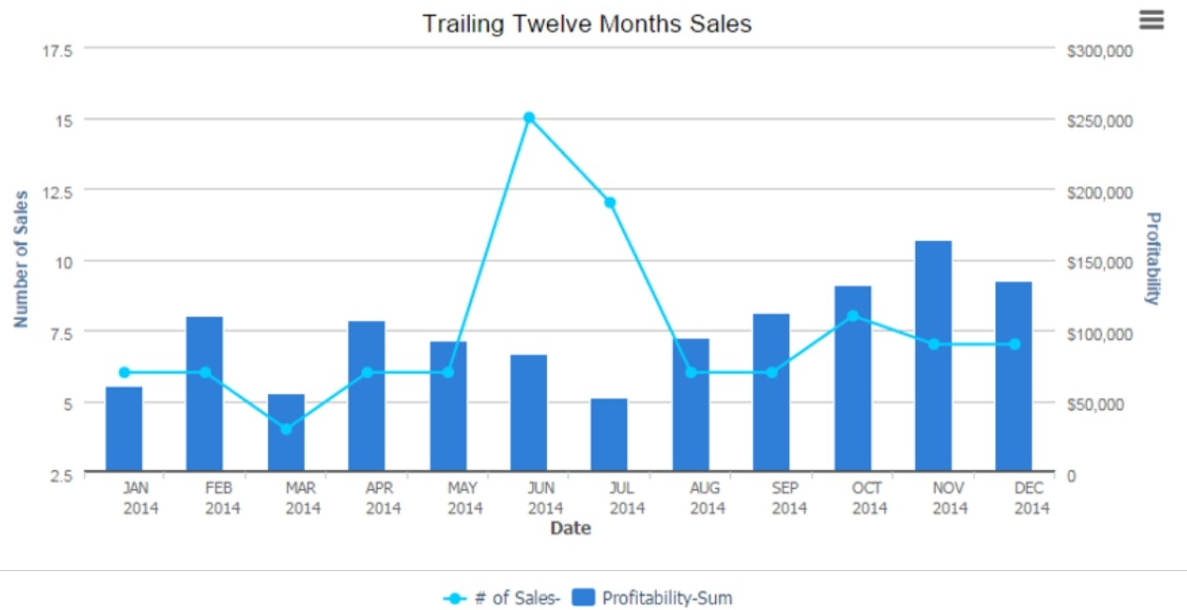
\includegraphics[width=0.85\linewidth]{img/di_trailing_sails.png}\end{center}
\ptesub{范文 Model Answer}
\begin{modelbox}
The following graph gives information about trailing twelve months sales. According to this graph, in January, the value of sales is around six. And in February, that of profitability sum is around eight, which is higher. The highest profitability sum is in November, around eleven. Finally, the lowest one of sales is in March, around four. In conclusion, June has the highest value of sales.
\end{modelbox}
\zh{下图给出的是过去十二个月销售额的信息。根据该图，一月份的销售额数值约为 6；二月份的盈利总额约为 8，数值更高。盈利总额的最高点在十一月，约为 11。最后，销售额的最低点在三月，约为 4。总之，六月的销售额数值最高。}
\ptesub{你的作答（AI 语音识别逐词配色）}
\asrlegend
\begin{asrbox}
\sg{this} \sg{graph} \sy{gives} \sg{information} \sg{about} \sg{training} \sr{twelve} \sy{month} \sy{sale} \sg{and} \sy{the} \sg{ex} \sg{accesses} \sy{data} \sr{and} \sr{the} \sy{y} \sr{axis} \sg{is} \sy{number} \sg{of} \sg{sale} \sg{and} \sg{we} \sg{can} \sg{see} \sy{the} \sy{lowest} \sy{one} \sg{is} \sy{in} \sy{the} \sy{july} \sg{two} \sy{thousand} \sg{and} \sg{forty} \sy{is} \sg{five} \sg{percent} \sg{and} \sg{we} \sg{can} \sg{see} \sy{the} \sg{largest} \sy{a} \sy{number} \sy{of} \sg{skills} \sy{is} \sy{in} \sg{november} \sy{two} \sy{thousand} \sg{and} \sg{forty} \sy{is} \sg{about} \sy{ten} \sg{percent} \sg{and} \sg{we} \sg{can} \sg{see} \sg{the} \sr{perfect} \sy{ibility} \sy{of} \sr{it} \sy{um} \sr{in} \sg{there} \sy{is} \sg{from} \sr{a} \sy{january} \sg{to} \sg{december} \sg{will} \sg{be} \sg{increasing} \sg{so}
\end{asrbox}
\smallskip
{\small\textbf{评分：}内容 \sfull{4.5/5} \quad\textperiodcentered\quad 发音 \sfull{71/90} \quad\textperiodcentered\quad 流利度 \spart{51/90}}\quad{\footnotesize\color{gray}（录音 0:40，用时 01:06）}
\end{qblock}

% ---------------- Q20 ----------------
\begin{qblock}{Q20\quad DI \#692\ \ Vehicle Sales}{描述图 · 总分 \textcolor{cAccent}{\bfseries 63}/90}
\ptesub{配图 Image}
\begin{center}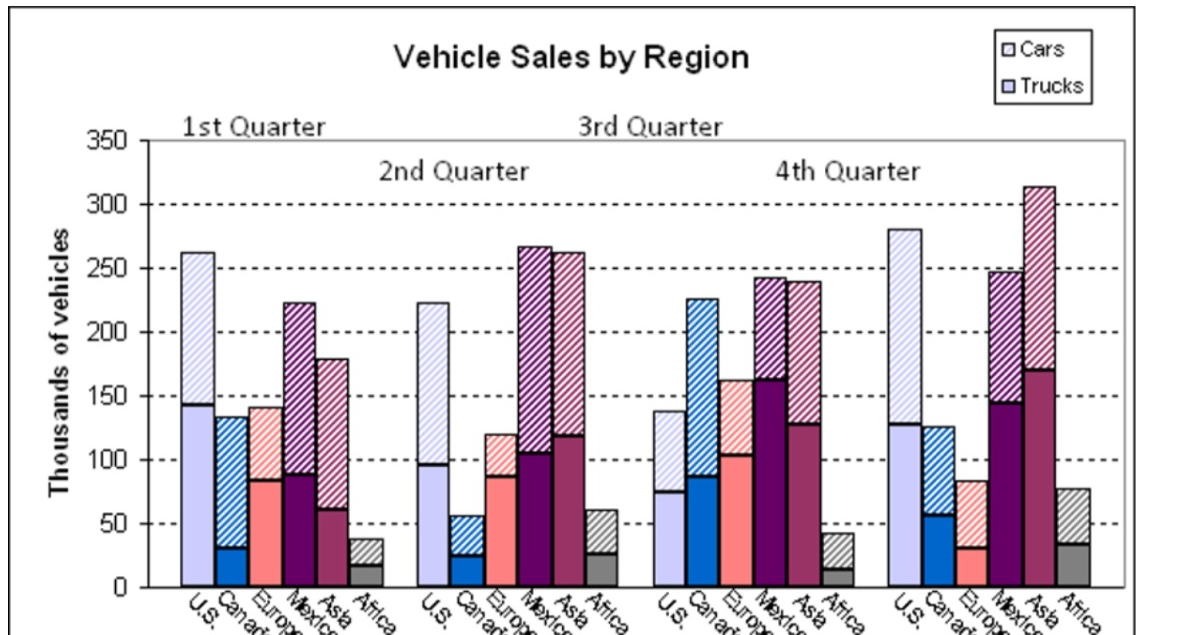
\includegraphics[width=0.85\linewidth]{img/di_vehicle_sales.png}\end{center}
\ptesub{范文 Model Answer}
\begin{modelbox}
The following graph gives information about vehicle sales by region. In the first quarter, the value of US is around two hundred and sixty, and that of Canada is lower, around one hundred and forty. The highest number of Asia is in the fourth quarter, which is three hundred and twenty. Finally, the highest one of Europe is in the third quarter. In conclusion, Africa has the lowest sales.
\end{modelbox}
\zh{下图给出的是各地区车辆销量的信息。第一季度，美国的数值约为 260，而加拿大的数值较低，约为 140。亚洲的最高数值出现在第四季度，为 320。最后，欧洲的最高值出现在第三季度。总之，非洲的销量最低。}
\ptesub{你的作答（AI 语音识别逐词配色）}
\asrlegend
\begin{asrbox}
\sg{we} \sg{can} \sg{see} \sy{the} \sg{following} \sg{graph} \sy{gives} \sg{information} \sg{about} \sg{vehicles} \sy{skill} \sg{by} \sg{religions} \sg{and} \sg{the} \sy{axis} \sy{accesses} \sy{is} \sy{religions} \sg{and} \sy{the} \sy{y} \sg{accesses} \sr{sound} \sy{of} \sy{vehicles} \sg{and} \sg{we} \sg{can} \sg{see} \sg{the} \sg{africa} \sg{is} \sg{always} \sr{the} \sy{smallest} \sg{one} \sg{and} \sy{the} \sy{max} \sr{nicole} \sy{and} \sg{asia} \sg{is} \sg{always} \sg{the} \sy{a} \sg{biggest} \sg{one} \sy{um} \sr{all} \sr{in} \sy{all} \sr{it's} \sg{a} \sy{vehicle} \sg{skill} \sg{by} \sg{regions} \sy{in} \sy{this} \sg{graph}
\end{asrbox}
\smallskip
{\small\textbf{评分：}内容 \sfull{4.5/5} \quad\textperiodcentered\quad 发音 \sfull{72/90} \quad\textperiodcentered\quad 流利度 \spart{56/90}}\quad{\footnotesize\color{gray}（录音 0:40，用时 01:06）}
\end{qblock}

% ---------------- Q21 ----------------
\begin{qblock}{Q21\quad DI \#690\ \ Man at Desk}{描述图 · 总分 \textcolor{cAccent}{\bfseries 59}/90}
\ptesub{配图 Image}
\begin{center}
\includegraphics[width=0.6\linewidth]{img/di_man_at_desk.png}\end{center}
\ptesub{范文 Model Answer}
\begin{modelbox}
The following graph gives information about a man sitting at a desk. In the central area, there is a desk with an open book on it; the color of the book is white. In the right area, it is a laptop with a black keyboard; the color of it is silver. The background has a big screen of a desktop, with a black frame. The weather is sunny. The man is sitting in the chair at the desk. To sum up, the graph tells about a man at the desk.
\end{modelbox}
\zh{下图给出的是一名男子坐在桌前的信息。在中间区域，桌上放着一本打开的书，书的颜色是白色。在右侧区域，是一台带黑色键盘的笔记本电脑，机身颜色是银色。背景中有一个大型台式电脑屏幕，边框是黑色的。天气晴朗，这名男子正坐在桌边的椅子上。总而言之，该图讲述的是一名男子在书桌前的情景。}
\ptesub{你的作答（AI 语音识别逐词配色）}
\asrlegend
\begin{asrbox}
\sg{we} \sg{can} \sg{see} \sg{the} \sy{following} \sy{graph} \sy{gives} \sg{information} \sg{about} \sy{a} \sg{man} \sg{who} \sg{is} \sy{a} \sy{using} \sy{his} \sg{computer} \sy{and} \sy{watching} \sg{his} \sg{book} \sg{we} \sg{can} \sg{see} \sy{the} \sy{man} \sy{is} \sy{where} \sr{a} \sy{two} \sr{to} \sy{a} \sy{t-shirt} \sg{and} \sy{on} \sy{the} \sg{central} \sg{of} \sg{the} \sg{graph} \sy{is} \sr{a} \sg{book} \sg{and} \sr{on} \sy{the} \sy{left} \sy{are} \sr{you} \sy{off} \sy{the} \sy{graph} \sy{we} \sg{can} \sy{see} \sy{three} \sg{computers} \sy{in} \sg{it} \sr{i'm} \sr{all} \sr{in} \sy{all} \sr{it's} \sy{a} \sy{photo} \sy{about} \sr{a} \sg{man} \sg{who} \sg{is} \sg{watching} \sg{his} \sy{books} \sy{and} \sg{watching} \sg{his} \sg{computer}
\end{asrbox}
\smallskip
{\small\textbf{评分：}内容 \sfull{4.3/5} \quad\textperiodcentered\quad 发音 \sfull{68/90} \quad\textperiodcentered\quad 流利度 \spart{58/90}}\quad{\footnotesize\color{gray}（录音 0:40，用时 01:06）}
\end{qblock}

\ptetask{情景应答}{Respond to a Situation · RTS　Q22--24（评分含恰当性）}
% ---------------- Q22 ----------------
\begin{qblock}{Q22\quad RTS (C) \#29\ \ Birthday Activity}{情景应答 · 总分 \textcolor{cAccent}{\bfseries 40}/90}
\ptesub{情景 Situation}
\begin{promptbox}
You're organizing a team outing to celebrate a colleague's birthday-Dave, and everyone's suggesting different activities. However, you realize that some options might not be suitable due to varying preferences and physical abilities. You need to gently guide the discussion towards inclusive activities that everyone can enjoy regardless of their interests or limitations. What would you say to your colleagues?
\end{promptbox}
\zh{你正在组织一次团队出游来庆祝同事戴夫（Dave）的生日，大家都在建议不同的活动。然而你意识到，由于每个人的偏好和身体条件不同，有些方案可能并不合适。你需要温和地把讨论引向那种不论兴趣或身体限制、人人都能享受的包容性活动。你会对同事们说什么？}
\ptesub{参考答案 Model Answer}
\begin{modelbox}
Hey team, I'm thrilled about planning our outing for Dave's birthday! Let's consider activities that everyone can participate in comfortably. How about we go for a picnic in the park or have a game night at someone's place? These options cater to various interests and physical abilities, ensuring everyone has a great time. Let's focus on creating inclusive and enjoyable memories together!
\end{modelbox}
\zh{嘿，团队们，我很期待为戴夫的生日筹划这次出游！让我们考虑那些每个人都能舒适参与的活动。不如我们去公园野餐，或者在某人家里搞一个游戏之夜？这些选择能兼顾各种兴趣和身体条件，确保每个人都玩得开心。让我们专注于一起创造包容而愉快的回忆吧！}
\ptesub{你的作答（AI 语音识别逐词配色）}
\asrlegend
\begin{asrbox}
\sy{hi} \sg{everyone} \sy{welcome} \sg{to} \sg{this} \sg{celebrating} \sg{'s} \sg{and} \sy{i} \sg{notice} \sg{that} \sy{a} \sg{everyone} \sy{suggest} \sg{different} \sg{activities} \sg{but} \sg{i} \sy{realize} \sg{that} \sg{some} \sg{options} \sg{might} \sg{not} \sg{be} \sg{suitable} \sg{due} \sg{to} \sy{very} \sy{preference} \sg{and} \sg{cycle} \sg{abilities} \sg{so} \sg{i} \sy{think} \sr{that's} \sr{a} \sy{can} \sg{join} \sg{the} \sr{a} \sr{a} \sy{discussion} \sr{is} \sy{of} \sy{their} \sg{interest} \sy{and} \sg{limitations} \sy{let's} \sg{have} \sg{a} \sg{good} \sg{time}
\end{asrbox}
\smallskip
{\small\textbf{评分：}恰当性 \spart{56/90} \quad\textperiodcentered\quad 发音 \spart{32/90} \quad\textperiodcentered\quad 流利度 \spart{40/90}}\quad{\footnotesize\color{gray}（录音 0:34，用时 01:29）}
\end{qblock}

% ---------------- Q23 ----------------
\begin{qblock}{Q23\quad RTS (C) \#30\ \ Group Presentation}{情景应答 · 总分 \textcolor{cAccent}{\bfseries 46}/90}
\ptesub{情景 Situation}
\begin{promptbox}
You're preparing for a group presentation, and your team members suggest incorporating complex charts and graphs into the slides. However, you realize that these visuals might confuse the audience and distract from the main points. You need to gently steer the discussion towards simpler and clearer visuals that enhance understanding. What would you say to your team members?
\end{promptbox}
\zh{你正在准备一次小组演示，团队成员建议在幻灯片中加入复杂的图表和图形。然而你意识到，这些视觉元素可能会让听众感到困惑，并分散他们对要点的注意力。你需要温和地把讨论引向更简单、更清晰、有助于理解的视觉呈现方式。你会对团队成员说什么？}
\ptesub{参考答案 Model Answer}
\begin{modelbox}
Hey guys, I appreciate the suggestion for the presentation slides. However, let's aim for simpler visuals to ensure our audience grasps the main points easily. How about we use straightforward charts and diagrams that highlight key information without overwhelming them? This way, we can enhance understanding and keep everyone engaged throughout the presentation. Let's prioritize clarity and effectiveness in our visuals.
\end{modelbox}
\zh{嘿，大家好，谢谢你们对演示幻灯片提出的建议。不过，让我们力求更简洁的视觉呈现，以确保听众能轻松抓住要点。不如我们使用简单明了的图表和示意图，突出关键信息又不让人应接不暇？这样一来，我们就能增进理解，让大家在整个演示过程中都保持专注。让我们把清晰和效果放在视觉设计的首位吧。}
\ptesub{你的作答（AI 语音识别逐词配色）}
\asrlegend
\begin{asrbox}
\sg{hey} \sg{guys} \sy{welcome} \sg{to} \sg{this} \sg{group} \sy{presentation} \sg{and} \sg{i} \sg{have} \sy{notice} \sy{you} \sg{are} \sg{suggesting} \sg{incorporating} \sy{complex} \sr{charts} \sy{and} \sg{graphs} \sg{into} \sg{the} \sg{slides} \sg{however} \sy{i} \sg{notice} \sy{that} \sy{this} \sg{visual} \sy{might} \sg{confuse} \sg{a} \sg{audience} \sg{and} \sy{distract} \sg{from} \sg{the} \sy{main} \sg{points} \sy{i} \sy{think} \sy{it's} \sg{make} \sg{this} \sy{discussions} \sy{over} \sg{the} \sg{simpler} \sy{and} \sg{clear} \sg{visual} \sg{than} \sy{in-house} \sg{understanding} \sg{let's} \sg{go}
\end{asrbox}
\smallskip
{\small\textbf{评分：}恰当性 \sfull{62/90} \quad\textperiodcentered\quad 发音 \spart{41/90} \quad\textperiodcentered\quad 流利度 \spart{43/90}}\quad{\footnotesize\color{gray}（录音 0:34，用时 01:28）}
\end{qblock}

% ---------------- Q24 ----------------
\begin{qblock}{Q24\quad RTS (C) \#31\ \ A Charity Event}{情景应答 · 总分 \textcolor{cAccent}{\bfseries 25}/90}
\ptesub{情景 Situation}
\begin{promptbox}
You're coordinating a charity event for your company, and your team proposes hosting a silent auction to raise funds. However, you realize that organizing the auction might require more resources and time than anticipated. You need to gently guide the discussion towards simpler fundraising ideas. What would you say to your team?
\end{promptbox}
\zh{你正在为公司统筹一场慈善活动，团队提议举办一场无声拍卖来筹款。然而你意识到，筹办这场拍卖可能需要比预想更多的资源和时间。你需要温和地把讨论引向更简单的筹款方案。你会对团队说什么？}
\ptesub{参考答案 Model Answer}
\begin{modelbox}
Hey team, I love the idea of a silent auction for our charity event, but let's consider simpler alternatives that are equally effective. How about organizing a bake sale or a raffle instead? These options require less time and resources to set up but still have the potential to raise significant funds for our cause. Let's brainstorm some creative ideas that align with our goals and resources.
\end{modelbox}
\zh{嘿，团队们，我很喜欢为我们的慈善活动办一场无声拍卖的想法，不过让我们考虑一些同样有效但更简单的替代方案吧。不如我们改为组织一场义卖蛋糕或抽奖活动？这些方案花费的时间和资源更少，却仍有可能为我们的事业筹到可观的善款。让我们一起头脑风暴一些既有创意、又契合我们目标和资源的点子吧。}
\ptesub{你的作答（AI 语音识别逐词配色）}
\asrlegend
\begin{asrbox}
\sg{hey} \sg{guys} \sy{thank} \sg{you} \sg{to} \sg{help} \sg{me} \sg{to} \sg{call} \sy{coordinate} \sy{or} \sy{clarity} \sg{events} \sy{of} \sg{our} \sg{company} \sg{but} \sg{i} \sg{have} \sg{realized} \sg{that} \sy{the} \sg{organizing} \sg{and} \sy{the} \sy{active} \sy{might} \sg{require} \sg{more} \sg{resources} \sg{and} \sg{the} \sy{time} \sr{than} \sy{anticipated} \sy{so} \sg{let's} \sg{make} \sg{the} \sg{discussion} \sr{towards} \sg{simpler} \sy{fundraise} \sg{ideas} \sy{i} \sg{think} \sg{that} \sy{we} \sg{can} \sg{make} \sy{our} \sg{company} \sy{a} \sy{good} \sr{i'm} \sy{more} \sy{and} \sy{more} \sg{healthy} \sy{um} \sy{so} \sg{let's} \sg{go} \sr{okay} \sr{okay}
\end{asrbox}
\smallskip
{\small\textbf{评分：}恰当性 \spart{41/90} \quad\textperiodcentered\quad 发音 \szero{18/90} \quad\textperiodcentered\quad 流利度 \spart{24/90}}\quad{\footnotesize\color{gray}（录音 0:38，用时 01:30）}
\end{qblock}

\ptetask{简短回答}{Answer Short Question · ASQ　Q25--30（单题 0/1）}
\begin{notebox}
{\footnotesize\color{gray}ASQ 考查听问答词，单题 0/1。你的录音不收；下表为题目、中文翻译与参考答案（绿）。}
\smallskip\par
\textbf{Q25\quad ASQ \#1391}\quad{\footnotesize\color{gray}（用时 00:16，得分 \szero{0/1}）}\\
What do we call the fabric that covers the floor of an apartment?\\
\zh{我们把覆盖公寓地板的织物叫做什么？}\\
参考答案：{\color{cFix}\textbf{Carpet / carpets}}（地毯）
\par\smallskip
\textbf{Q26\quad ASQ \#1390}\quad{\footnotesize\color{gray}（用时 00:18，得分 \szero{0/1}）}\\
What do we call the room that is below the level of the ground?\\
\zh{我们把低于地面水平的房间叫做什么？}\\
参考答案：{\color{cFix}\textbf{Basement / cellar}}（地下室 / 地窖）
\par\smallskip
\textbf{Q27\quad ASQ \#1385}\quad{\footnotesize\color{gray}（用时 00:19，得分 \szero{0/1}）}\\
What do we usually call a person who is receiving medical treatment in a hospital?\\
\zh{我们通常把在医院接受治疗的人叫做什么？}\\
参考答案：{\color{cFix}\textbf{Patient / patients}}（病人）
\par\smallskip
\textbf{Q28\quad ASQ \#1384}\quad{\footnotesize\color{gray}（用时 00:18，得分 \szero{0/1}）}\\
Which piece of equipment is used to control the direction of ships?\\
\zh{哪种设备是用来控制船只方向的？}\\
参考答案：{\color{cFix}\textbf{Rudder / rudders}}（舵）
\par\smallskip
\textbf{Q29\quad ASQ \#1382}\quad{\footnotesize\color{gray}（用时 00:18，得分 \szero{0/1}）}\\
Which one is a psychologist good at, surgery or therapy?\\
\zh{心理学家更擅长哪一项，外科手术还是心理治疗？}\\
参考答案：{\color{cFix}\textbf{Therapy}}（心理治疗）
\par\smallskip
\textbf{Q30\quad ASQ \#1381}\quad{\footnotesize\color{gray}（用时 00:18，得分 \szero{0/1}）}\\
What do we call the vacation taken by a couple who have just got married?\\
\zh{我们把新婚夫妇度的假叫做什么？}\\
参考答案：{\color{cFix}\textbf{Honeymoon}}（蜜月）
\end{notebox}

\end{document}
